\en

\section{Participant Observation Experiment}

For our initial participant observation, we attempted to mitigate two code duplications found by ArKanjo tool
in the AMD Display driver applying our systematic approach presented in \ref{subsubsec:systematic}. 
As presented in section \ref{sec:meteth}, we opted for applying the systematic approach in the functions 
\textit{offset\_to\_id} and \textit{phy\_id\_to\_atom} in the folders \textit{dc/gpio} and \text{dc/bios} respectively.

Hereafter, the mitigation on \textit{offset\_to\_id} will be referred to as mitigation 1, and the mitigation on 
\textit{phy\_id\_to\_atom} will be referred to as mitigation 2. Table \ref{tab:patch} summarizes the impact of the mitigations
in terms of files and lines changed, and the refactoring method used. We present our experience and learning for each mitigation 
in the next sections.

\begin{table}
\begin{tabular}{ | c | c | c | c | m{6em} | }

\hline

\textbf{Mitigation} & \textbf{Files changed} & \textbf{Lines added} & \textbf{Lines removed} & \textbf{Refactoring methods used}
\\ \hline 

1 & 13 & +224 & -753 & Parameterize Method, Extract Method  \\ \hline
2 & 8 & +132 & -517 & None \\ \hline

\hline
\end{tabular}
\caption{Early results on mitigating code duplications on the AMD Display driver.}
\label{tab:patch}
\end{table}


\subsection{Mitigation 1}

On the process of the systematic approach, we found that the \textit{offset\_to\_id} function exist in code 10 files, enclosing
multiple GPU architectures. The duplicated functions are not exactly equals, as there are some minimal specific logics applied
to each GPU architecture. To address this issue, we applied the extract method to break the function in smaller parts and the 
parameterize method to address the specific logics for the GPU's.

We reached a point with a scratch on how we would mitigate the duplications found were done, but we could not complete the refactoring on a state 
capable to submit as a patch to the driver. 
We found that the configuration files on the AMD Display driver are designed to be imported at compilation time
using \textit{\#define} macros. The configuration files design choice makes the refactoring of duplications on generic 
approachs trickier, as refactoring code that depends on these files requires significant refactor on the configuration files
design and deep knowledge of the codebase, which us as first-timer contributors do not have. Thus, we opted to not continue 
on investigating this mitigation.

\subsection{Mitigation 2}

On the process of the systematic approach, we found that the \textit{phy\_id\_to\_atom} function exist in 5 code files, and 
there are two other functions that are duplicated on those 5 code files, which . All functions across the files were
exactly equal, thus there was no need to apply refactor methods presented in literature. The refactoring work was resumed
to creating a generic library and fixing the compilation targets. 

The code files touched in the second mitigation does 
not depend on configuration files, thus we have not faced the same issues on the first mitigation. 
The refactoring of the code to mitigate duplications reached a point we judged that was good enough to submit as a patch
to contribute to the AMD Display driver code quality. Thus we moved to send the refactoring to the driver's maintainers 
as patch, documenting or findings and experiences on the process.

\begin{figure}
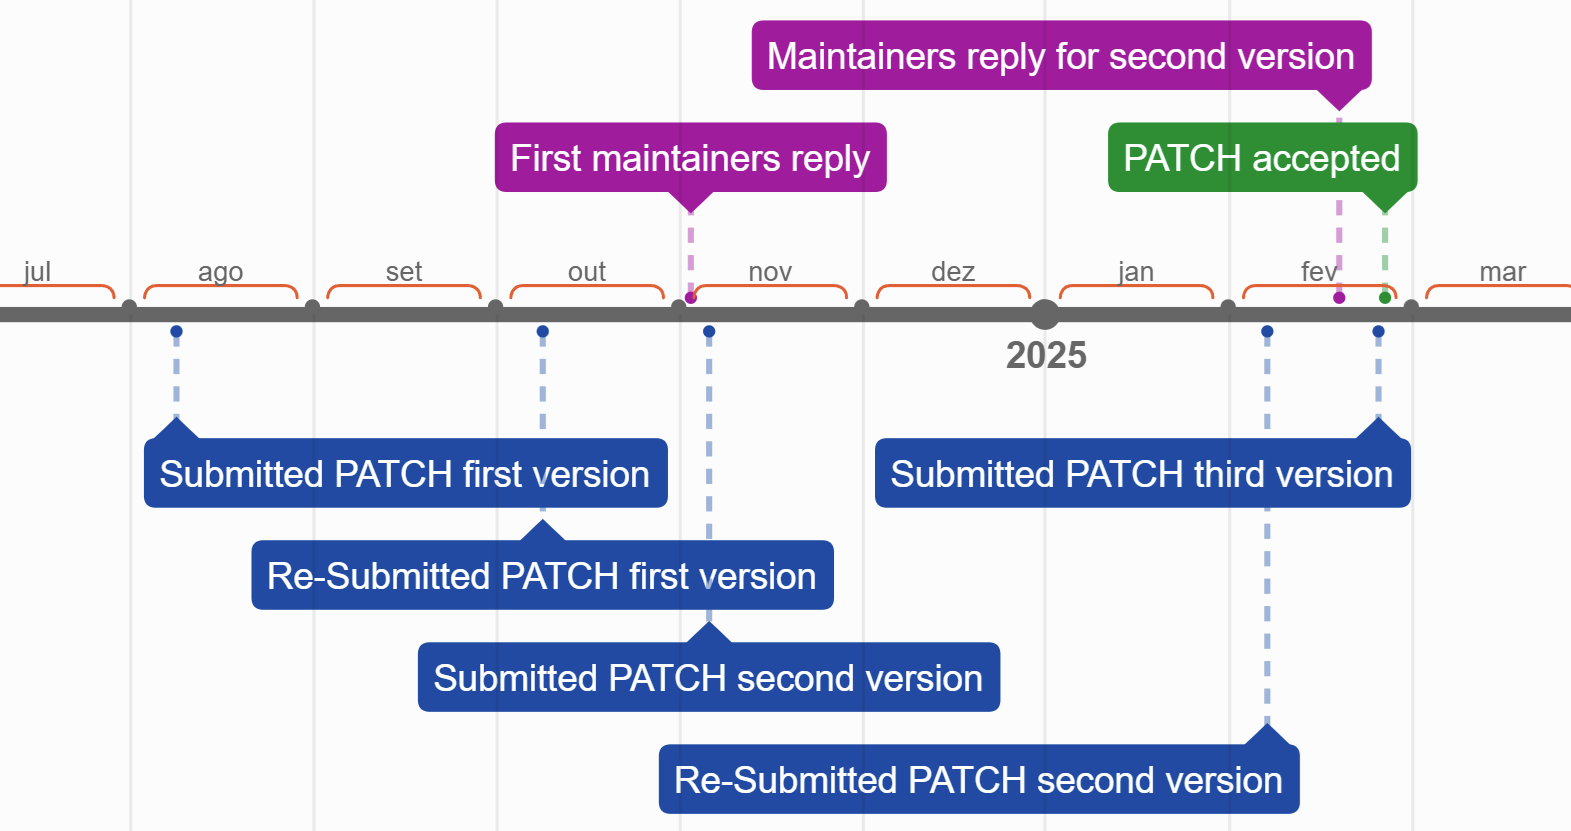
\includegraphics[scale=0.45]{timeline_patch}
\caption{Timeline of the PATCH submission process}
\label{fig:timeline}
\end{figure}

The experience on submiting a patch was not as we expected.
The overall process took 7 months and 16 days, which is a time significant slower then we expected.
We initially submitted the patch on Auguest 9th, 2024, but we did not receive replies at first. Thus, we had
to to resend it on October 9th 2024. We received an initial response on November 3rd, 2024 asked for minimal changes, 
we submitted a second version with the changes request on November 16th, 2024. We did not receive replies
at first and need to resend the patch on February 7th, 2025. 
We received a reply on February 11th 2025 asking for additional changes. 
We sent an third version on February 24th 2025 and the patch got accepted and integrated in the kernel codebase in 
February 25th 2025. Figure \ref{fig:timeline} illustrate the timeline of the patch submission.

We discussed with our point of contact at the AMD Display driver to understand the reason of the slow process
to submit a patch. 
We learned that some of the code in the driver is shared across all operating systems that 
support the implemented GPUs. 
This fact creates a complex process within AMD to format and submit changes across the supported systems while 
simultaneously implementing measures to mitigate errors.
Additionally, we comprehended that AMD Display driver developers can not view duplicated code negatively, 
as we understand it is a good practice in software engineering. One example shared with us is that duplicated 
code enhances the independence of GPU driver code, allowing developers to make changes to a specific GPU without 
needing to test compatibility with others. This approach helps save significant time and effort. 

Regarding the patch changes requested for the second version, 
only minor changes were requested to align with code style, license correct use and best practices that
were initially unkown to use. For the change requested on the third version, we were simple asked to 
move the functions created in the generic library to a existent file, instead of creating a new one.
More details of the patch can be found in Appendix \ref{app:feedback} and the patch submitted in 
the linux codebase can be see here: \url{https://lore.kernel.org/all/20250225015532.303032-1-luanicaro@usp.br/}.

The initial plan of this research was to approach and sent a large number of mitigations to
collect a broad number of artifacts from the driver community, but the slow process to send a patch
makes this plan unviable. Thus, we opted to redirect this research to work with students and refactoring duplicated function
pairs found by the tool directly in the IIO and the AMD Display driver, without passing through the whole process 
of the systematic approach proposed.
This alternative allowed us to collect artifacts from the students experiences and findings, and not be 
to dependable of the iteraction with the kernel community.
A additional advantage is to accelerate the iteraction with the kernel community
because we are not applying the systematic approach, which translate to smaller code changes.
